\chapter{Huidige situatie}

\label{Chapter4}

Dit hoofdstuk gaat over de deelvraag \enquote{\deelhuidig}

\section{Huidige Architectuur}
De huidige website is een combinatie van een PHP \& Symfony back-end API en Content Management Systeem, samen met een React + next.js front-end. De infrastructuur is momenteel gebouwd op Docker(-compose) + Ansible. Bitbucket pipeline wordt gebruikt voor het Continuous Integration / Deployment. 

In figuur \ref{fig:infra} is een component diagram te vinden van de huidige website structuur. De front-en backend structuur bevat 5 docker containers:
\begin{itemize}
	\item \textbf{PHP-FPM} (back-end)
	\item \textbf{Nginx} (front-en backend)
	\item \textbf{Redis} (back-end)
	\item \textbf{NodeJS} (front-end)
	\item \textbf{PostgreSQL} (back-end)
\end{itemize}

\begin{figure}
	\centering
	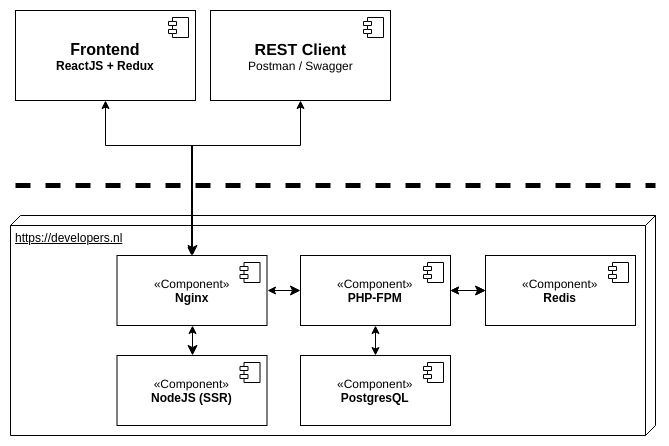
\includegraphics[width=13cm]{Figures/Infrastructure}
	\decoRule
	\caption[Infrastructuur]{Infrastructuur website front-en backend \parencite{Documentation}}
	\label{fig:infra}
\end{figure}

PHP-FPM is een FastCGI Process Manager, deze Container serveert de Symfony “FosREST” API en het Content Management Systeem. De NodeJS container serveert een statische Next.js React applicatie en maakt gebruik van Server Side Rendering. Er zit een Nginx reverse proxy in die kiest om een request naar de back-end of de front-end te laten gaan. Redis is een Key-Value Database die gebruikt wordt voor het cachen, en een PostgreSQL container als database. De Bitbucket Pipeline gebruikt Ansible om op de servers de geüpdatete containers te pullen en te starten.

Voor zowel de front- als backend is één monitoring tool genaamd \enquote{Sentry} geïmplementeerd. Sentry creëert een duidelijk overzicht voor alle errors die opkomen in productie.

Ook heeft Developers.nl een \enquote{Employee Management Systeem} (EMS) gebouwd. Deze heeft een soortgelijke structuur aan de website. Het EMS bevat zeer veel gevoelige informatie en het is dus van hoog belang dat deze goed beveiligd is.

\section{Metingen}

Nu de infrastructuur in kaart is gebracht luidt de vraag; hoe schaalbaar is deze infrastructuur eigenlijk? Om dit te beantwoorden worden de verschillende definities van schaalbaarheid individueel behandeld.

\subsection{Structural scalability}
Definitie: Het vermogen van een systeem om uit te breiden in een gekozen dimensie zonder ingrijpende wijzigingen in de architectuur.

Bij structural scalability hoort factor 3 (Config) van de 12-factor app. Een test om te bewijzen dat alle configuratie correct uit de code is verwerkt, is of de applicatie op elk gewenst moment open-source kan worden gemaakt zonder geclassificeerde informatie vrij te geven.

Voor de website wordt er gebruik gemaakt van docker-secrets en ansible-vault. Deze combinatie zorgt ervoor dat er nooit wachtwoorden, API sleutels en dergelijke plain-text in versiebeheer komt te staan. Deze secrets worden uiteindelijk in de containers als environment variabelen opgeslagen en uitgelezen door Symfony. In het EMS is deze techniek nog niet gebruikt en staan credentials wél plaintext in de repository.

Om aan factor 3 van de 12-factor app te voldoen moeten de configuratiefiles niet per specifieke omgeving (productie, test, staging) gegroepeerd worden maar moeten juist individueel per deployment geregeld worden. Dit gebeurt in zowel het EMS als de website, de bitbucket pipeline heeft zijn eigen specifieke environment variabelen om te gebruiken en de variabelen in de docker containers worden meegegeven in de algemene docker-compose file die in elke deployment hetzelfde zal zijn.

\subsection{Load scalability}
Definitie: Het vermogen van een systeem om elegant te presteren naarmate het aangeboden verkeer toeneemt. Om een load-test uit te voeren zijn meerdere tools met elkaar vergeleken:
\begin{itemize}
	\item https://loader.io/
	\item https://gatling.io/
	\item https://k6.io/
	\item http://tsung.erlang-projects.org/
\end{itemize}

De gratis versie van loader.io is niet genoeg voor de wensen van de test, voor gatling.io is Ruby kennis nodig, en voor Tsung worden de tests in XML geschreven wat het lastig maakt om de load op te schalen. Uiteindelijk is gekozen voor K6 omdat zo goed als elke ontwikkelaar genoeg Javascript kennis heeft om deze tool te gebruiken. Ook heeft k6 een gemakkelijke manier om de hoeveelheid Virtual Users (VU) geleidelijk te verhogen. Om de uitkomsten te visualiseren is InfluxDB samen met Grafana gebruikt. In bijlage \ref{Bijlagek6} is de implementatie hiervan te vinden.

Bij load scalability horen factor 6 \textbf{(processes)}, 8 \textbf{(concurrency)} en 9 \textbf{(disposability)} van de 12-factor app methodologie. Factor 6 vereist dat de applicatie als één of meerdere \enquote{stateless processes} moet uitgevoerd worden. Bij de PHP containers worden geüploade bestanden weggeschreven naar een volume, dit zorgt ervoor dat de container niet volledig stateless meer is. Ook zijn databases in docker containers geplaatst, dit is een stateful process aangezien het van belang is dat niet alle data verloren gaat zodra de container stopt.

Voor factor 8 \textbf{(concurrency)}......

Voor factor 9 \textbf{(disposability)} moet een applicatie opstarttijd minimaliseren. Zodra de docker images de initiële buildtime voorbij zijn kan de applicatie snel uit en aan worden gezet. \textcolor{red}{TODO: HOE SNEL?} % TODO: Hoe snel?

Ook vereist factor 9 dat processen netjes worden afgesloten zodra ze een \texttt{SIGTERM} ontvangen. Zodra een docker container met \texttt{docker stop <container>} gestopt wordt zal er een SIGTERM worden gestuurd naar de draaiende processen. De vier containers met processen zijn PostgreSQL, PHP-FPM, Nginx en Redis. Deze sluiten allemaal netjes af en hebben de volgende outputs zodra ze worden gestopt:

\subsubsection{PostgreSQL}
\begin{minted}{text}
LOG: received smart shutdown request
LOG: background worker "logical replication launcher" (PID 43) exited with exit code 1
LOG: shutting down
LOG: database system is shut down
\end{minted}

\subsubsection{PHP-FPM}
\begin{minted}{text}
NOTICE: Terminating ...
NOTICE: exiting, bye-bye!
\end{minted}

\subsubsection{Redis}
\begin{minted}{text}
1:signal-handler (1570781278) Received SIGTERM scheduling shutdown...
# User requested shutdown...
* Saving the final RDB snapshot before exiting.
* DB saved on disk
* Removing the pid file.
# Redis is now ready to exit, bye bye...
\end{minted}

\subsubsection{Nginx}
\begin{minted}{text}
[notice] 1#1: signal 15 (SIGTERM) received from 56, exiting
[notice] 48#48: exiting
[notice] 47#47: exiting
[notice] 47#47: exit
[notice] 1#1: signal 14 (SIGALRM) received
[notice] 1#1: signal 17 (SIGCHLD) received from 48
[notice] 1#1: cache manager process 48 exited with code 0
[notice] 1#1: worker process 47 exited with code 0
[notice] 1#1: exit
\end{minted}

Ook moeten de processen bestendig zijn tegen \enquote{sudden death}. Om dit te simuleren kan \texttt{docker kill <container>} gebruikt worden om een \texttt{SIGKILL} te sturen naar de hoofdprocessen. Hieronder is te zien dat alle containers na een \texttt{docker kill} zonder problemen weer kunnen opstarten.

\begin{minted}{text}
-  developers.nl git:(develop) docker ps -q
d0829783af18
f72e9967771b
01dd48ff5a59
fab794731d47
ca510c065d11
3ee85578efb5
-  developers.nl git:(develop) docker kill $(docker ps -q) 
docker ps
d0829783af18
f72e9967771b
01dd48ff5a59
fab794731d47
ca510c065d11
3ee85578efb5
-  developers.nl git:(develop) docker ps -q

-  developers.nl git:(develop) docker start $(docker ps -aq)
d0829783af18
f72e9967771b
01dd48ff5a59
fab794731d47
d68d7ab9809c
ca510c065d11
3ee85578efb5
e1866ab6c1af
-  developers.nl git:(develop) docker ps -q
d0829783af18
f72e9967771b
01dd48ff5a59
fab794731d47
ca510c065d11
3ee85578efb5
\end{minted}

\subsection{Functional scalability}
Definitie: In welke mate bestaande code moet worden aangepast zodra een nieuwe functionaliteit wordt toegevoegd aan het systeem.

Binnen de scope van de infrastructuur.

\subsection{Onderhoudbaarheid}
Definitie: The degree of effectiveness and efficiency with which a product or system can be modified to improve it, correct it or adapt it to changes in environment, and in requirements.

\section{conclusie}
